

\section{RBF-Networks}


\begin{frame}\frametitle{\secname}

A tradeoff between $k$NN classification and Parzen window classification.

Instead of taking all $p$ points to predict the class probabilities (Parzen), limit the prediction to $k \ll p$ \cancel{points} ``representative'' functions.

Represent all points $\vec x$ in terms of basis functions $\phi_i(\vec x), i=1\,\ldots,k$

Let $k$ be the number of basis functions.

\end{frame}

\begin{frame}

\begin{figure}[ht]
     \centering
     \savebox{\imagebox}{
	 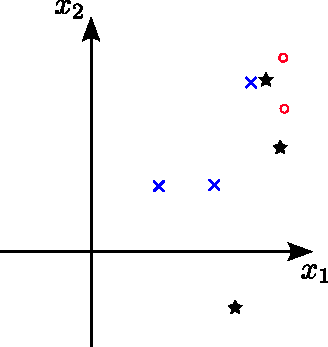
\includegraphics[width=0.37\textwidth]{img/parzen_data}}%
     \begin{subfigure}[t]{0.37\textwidth}
         \centering
         \usebox{\imagebox}% Place largest image
         \caption{Two-class data in 2D}
         \label{fig:quadratic}
     \end{subfigure}
     \hspace{2mm}
     \begin{subfigure}[t]{0.37\textwidth}
         \centering
         \raisebox{\dimexpr.5\ht\imagebox-.5\height}{% Raise smaller image into place
         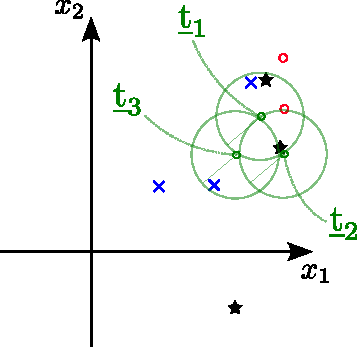
\includegraphics[width=0.99\textwidth]{img/rbf-network}
         }
         \caption{$k=3$ ``representatives''}
         \label{fig:rbf-network}
     \end{subfigure}
\end{figure}

\end{frame}

\subsection{Recap: Regression on transformed data}

\begin{frame}\frametitle{\subsecname}



\end{frame}
